\chapter{Time}

These aspects have been already mentioned, but let's recall some Time-related issues in distributed systems:
\begin{itemize}
   \item No global clock, every node has its own
   \item Asynchronous best-effort communication, messages may be lost
   \item No central authority, but coordination is needed
\end{itemize}

Time is fundamental for two reasons:
\begin{enumerate}
   \item \textbf{Ordering}: to order events, we need to know when they happened
   \item \textbf{Causal Relationships}: to determine cause-effect relationships, we need to know when they happened
   \item Handle \textbf{inconsistencies} between nodes
   \item Handle \textbf{conflicts}, such as multiple updates to a shared resource
\end{enumerate}

Going a bit deeper, there are distributed systems which are highly time-dependant:
\begin{itemize}
   \item Distributed \textbf{databases} - data must be consistent and transactions must either entirely succeed or entirely fail
   \item \textbf{IoT} systems - issuing commands to devices may be related to measurements taken at a certain time, besides, command receival and execution is always time-sensitive (e.g. suppose you get a ``turn left'' command too late)
   \item Cloud computing \textbf{auto-scaling} and \textbf{load balancing} - if you measure that the need for resources is increasing and you instance more VMs, but actually the need measurement is 2 hours old, you wasted resources and \textit{money}
\end{itemize}


\section{Challenges}
First of all, \textbf{Clock Drift} is one the key problems.
Every machine has its own \textit{phyisical} clock, which may gradually drift over time due to hardware imperfections.
It matters because over time, unsynchronized clocks on different nodes will show different times, leading to inconsistent timestamps for events.

Also \textbf{network latencies} are an issue
Messages between nodes can be delayed due to network congestion, causing events to be perceived in a different order than they occurred.

\subsection{NTP and PTP - Protocols Solving Drift}
\begin{paracol}{2}
   Network Time Protocol (NTP) is a protocol used to synchronize the clocks of computers over a network.

   It works on stratum levels, where a stratum 0 device is a reference clock, a stratum 1 device is a server that gets time from a stratum 0 device, and so on up to stratum 15.
   
   NTP can synchronize clocks to within milliseconds over the internet, but it is insufficient for environments needing higher precision.
   \switchcolumn
   \begin{figure}[htbp]
      \centering
      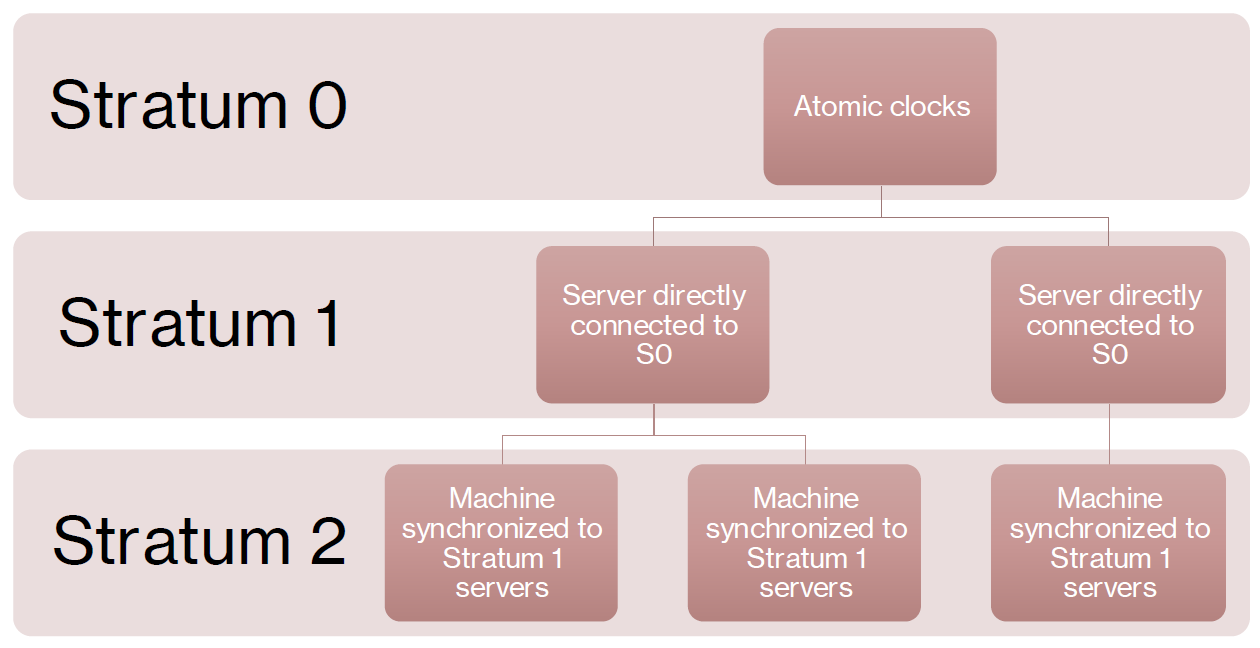
\includegraphics{images/03/ntp.png}
      \caption{NTP Stratum architecture}
      \label{fig:03/ntp}
   \end{figure}
\end{paracol}

PTP (Precision Time Protocol) is a protocol used to synchronize clocks in a network with sub-microsecond accuracy. Typically used in high-frequency trading, telecommunications, and industrial automation.

P TP uses a master-slave architecture, with a grandmaster clock providing time to all slaves.
PTP timestamps are often hardware- assisted for higher precision (e.g., using Network Interface Cards (NICs) with timestamping capabilities)

\note{In future lessons theses two protocols will be covered in more detail}

\subsection{Logical and Phyisical Clocks}
Logical clocks do not represent the actual time, but they are used to order events in a distributed system, ensuring that causally related events are ordered correctly even if the actual phyisical clocks are not synchronized.\\
Common examples are Lamport timestamp and vector clocks.